\documentclass[11pt]{article}

\usepackage[a4paper, margin=2.54cm]{geometry}

\usepackage{CJK}
\usepackage{amsmath}
\usepackage{graphicx}
\usepackage{siunitx}

\usepackage{tikz}
\usetikzlibrary{arrows.meta, positioning, calc, fit, decorations.pathreplacing}

\usepackage{array,tabularx}
\newcolumntype{L}[1]{>{\raggedright\arraybackslash}p{#1}}

\begin{document}
\begin{CJK}{UTF8}{gbsn}

\title{PLAN}

\maketitle

\section{kelmarsh 数据集，World Model Protocol}

kelmarsh 数据集一共有 6 台风机，每个数据间隔 10 分钟。

\paragraph{预测量：}\texttt{target\_kw} 机组 10 分钟平均发电功率，对应原始字段 \texttt{Power (kW)}。

\medskip

\noindent \textbf{本地机组观测：}

\noindent
\renewcommand{\arraystretch}{1.15}
\begin{tabularx}{\linewidth}{@{}L{6cm}L{0.6cm}L{2.5cm}L{3.5cm}L{4cm}X@{}}
Wind speed ($m/s$)                            && 风速       & wind\_direction\_sin & 风向           \\
Rotor speed (RPM)                             && 主轴转速   & wind\_direction\_cos & 风向           \\
Generator RPM (RPM)                           && 发电机转速 & yaw\_error\_sin      & 朝向与风向误差 \\
Nacelle ambient temperature (\SI{}{\celsius}) &\(T^{amb}\)& 环境温度   & yaw\_error\_cos      & 朝向与风向误差 \\
Nacelle temperature (\SI{}{\celsius})         &\(T^{nac}\)& 机内温度   & pitch\_mean          & 叶片转角均值   \\
\end{tabularx}

\medskip

\noindent \textbf{已知未来日历特征：}

\noindent
\renewcommand{\arraystretch}{1.15}
\begin{tabularx}{\linewidth}{@{}L{4.5cm}L{0.6cm}L{2.5cm}L{3.5cm}L{0.6cm}L{4cm}X@{}}
calendar\_hour\_sin    & & 日内时间编码 & calendar\_hour\_cos    & & 日内时间编码 \\
calendar\_weekday\_sin & & 星期周期编码 & calendar\_weekday\_cos & & 星期周期编码 \\
calendar\_month\_sin   & & 月份周期编码 & calendar\_month\_cos   & & 月份周期编码 \\
calendar\_is\_weekend  & & 是否周末     &                        & &              \\
\end{tabularx}

\medskip

\noindent \textbf{机组静态属性：}

\noindent
\renewcommand{\arraystretch}{1.15}
\begin{tabularx}{\linewidth}{@{}L{4.5cm}L{0.6cm}L{2.5cm}L{3.5cm}L{0.6cm}L{4cm}X@{}}
turbine\_id          & & 机组编号       & turbine\_index       &     & 机组索引     \\
latitude             & & 纬度           & longitude            &     & 经度         \\
coord\_x             & & 平面坐标 $x$   & coord\_y             &     & 平面坐标 $y$ \\
coord\_kind          & & 坐标类型       & coord\_crs           &     & 坐标参考系   \\
elevation\_m         & & 海拔           & rated\_power\_kw     &     & 额定功率     \\
hub\_height\_m       & & 轮毂高度       & rotor\_diameter\_m   & $D$ & 叶轮直径     \\
\end{tabularx}

\medskip

\noindent \textbf{机组对几何特征：}

\noindent
\renewcommand{\arraystretch}{1.15}
\begin{tabularx}{\linewidth}{@{}L{4.5cm}L{0.6cm}L{2.5cm}L{3.5cm}L{0.6cm}L{4cm}X@{}}
src\_turbine\_id               &            & 源机组编号    & dst\_turbine\_id       &             & 目标机组编号  \\
src\_turbine\_index            &            & 源机组索引    & dst\_turbine\_index    &             & 目标机组索引  \\
delta\_x\_m                    & $\Delta x$ & 水平 $x$ 位移 & delta\_y\_m            & $\Delta y$  & 水平 $y$ 位移 \\
distance\_m                    & $d$        & 机组间距离    & bearing\_deg           & $\beta$     & 机组间方位角  \\
distance\_in\_rotor\_diameters & $d^{(RD)}$ & 归一化距离    & elevation\_diff\_m     & $\Delta{h}$ & 海拔差        \\
\end{tabularx}

\medskip

\noindent \textbf{本地机组状态事件观测：}

\noindent
\renewcommand{\arraystretch}{1.15}
\begin{tabularx}{\linewidth}{@{}L{4cm}L{3.5cm}L{4cm}L{5cm}X@{}}
evt\_any\_active              & 是否有事件激活   & evt\_active\_count              & 激活事件数       \\
evt\_total\_overlap\_seconds  & 事件重叠秒数     & evt\_stop\_active               & 停机事件是否激活 \\
evt\_warning\_active          & 警告事件是否激活 & evt\_informational\_active      & 信息事件是否激活 \\
\end{tabularx}

\medskip

\noindent \textbf{场级观测}：

\noindent
\renewcommand{\arraystretch}{1.15}
\begin{tabularx}{\linewidth}{@{}L{5.75cm}L{0cm}L{2.4cm}L{4.8cm}L{5cm}X@{}}
farm\_pmu\_\_gms\_current\_a             & $I$ & 场级电流       & farm\_evt\_any\_active             & 场级是否有事件激活 \\
farm\_pmu\_\_gms\_power\_kw              & $P$ & 场级有功功率   & farm\_evt\_active\_count           & 场级激活事件数     \\
farm\_pmu\_\_gms\_reactive\_power\_kvar  & $Q$ & 场级无功功率   & farm\_evt\_total\_overlap\_seconds & 场级事件重叠秒数   \\
farm\_evt\_stop\_active                  &     & 场级停机事件   & farm\_evt\_warning\_active         & 场级警告事件       \\
farm\_evt\_informational\_active         &     & 场级信息事件   &                                    &                    \\
\end{tabularx}

\medskip

\paragraph{可用性 mask：} 所有 mask 均为 \texttt{int8}，取值 $1$ 表示对应 value 不可用，$0$ 表示可用。目标历史使用 \texttt{target\_kw\_\_mask}；所有本地机组观测和场级观测均使用 \texttt{<value\_column>\_\_mask} 作为 companion mask。

\noindent
\renewcommand{\arraystretch}{1.15}
\begin{tabularx}{\linewidth}{@{}L{4.2cm}L{3.5cm}L{5.2cm}L{4.3cm}X@{}}
target\_kw\_\_mask           & 目标功率可用性     & Rotor speed (RPM)\_\_mask    & 主轴转速可用性 \\
Wind speed (m/s)\_\_mask     & 风速可用性         & Generator RPM (RPM)\_\_mask  & 发电机转速可用性 \\
wind\_direction\_sin\_\_mask & 风向编码可用性     & evt\_any\_active\_\_mask     & 本地事件可用性 \\
wind\_direction\_cos\_\_mask & 风向编码可用性     & evt\_active\_count\_\_mask   & 本地事件数可用性 \\
yaw\_error\_sin\_\_mask      & 偏航误差可用性     & evt\_stop\_active\_\_mask    & 本地停机事件可用性 \\
yaw\_error\_cos\_\_mask      & 偏航误差可用性     & evt\_warning\_active\_\_mask & 本地警告事件可用性 \\
pitch\_mean\_\_mask          & 叶片转角均值可用性 & evt\_informational\_active\_\_mask & 本地信息事件可用性 \\
                             &                    & evt\_total\_overlap\_seconds\_\_mask & 本地事件重叠秒数可用性 \\
\end{tabularx}

\noindent
\renewcommand{\arraystretch}{1.15}
\begin{tabularx}{\linewidth}{@{}L{7cm}X@{}}
Nacelle ambient temperature (\SI{}{\celsius})\_\_mask & 环境温度可用性 \\
Nacelle temperature (\SI{}{\celsius})\_\_mask         & 机内温度可用性 \\
farm\_evt\_total\_overlap\_seconds\_\_mask            & 场级事件重叠秒数可用性 \\
farm\_evt\_informational\_active\_\_mask              & 场级信息事件可用性 \\
farm\_pmu\_\_gms\_reactive\_power\_kvar\_\_mask       & 场级无功功率可用性 \\
farm\_pmu\_\_gms\_current\_a\_\_mask                  & 场级电流可用性 \\
farm\_pmu\_\_gms\_power\_kw\_\_mask                   & 场级有功功率可用性 \\
farm\_evt\_any\_active\_\_mask                        & 场级事件可用性 \\
farm\_evt\_active\_count\_\_mask                      & 场级事件数可用性 \\
farm\_evt\_stop\_active\_\_mask                       & 场级停机事件可用性 \\
farm\_evt\_warning\_active\_\_mask                    & 场级警告事件可用性 \\
\end{tabularx}


\medskip

\noindent \textbf{序列标识与 farm-synchronous 审计字段：}

\noindent
\renewcommand{\arraystretch}{1.15}
\begin{tabularx}{\linewidth}{@{}L{2cm}L{4cm}L{4cm}L{5cm}X@{}}
\texttt{dataset}             & 数据集编号               & farm\_turbines\_expected     & 场内应有机组数           \\
turbine\_id                  & 机组编号                 & farm\_turbines\_with\_target & 当前时间有目标值的机组数 \\
quality\_flags               & 目标质量标记             & feature\_quality\_flags      & 特征质量标记             \\
timestamp                    & 时间戳                   & farm\_turbines\_observed     & 当前时间观测到的机组数   \\
is\_observed                 & 当前机组行是否观测到     & farm\_is\_fully\_synchronous & farm 时间点是否完全同步  \\
                             &                          & farm\_has\_all\_targets      & 是否所有机组都有目标值   \\
\end{tabularx}

\subsection{v1 数据契约（固定 schema）}

为避免实现阶段因特征选择、时间对齐或缩放方式不同而出现“同一网络、不同数据世界”的问题，v1 版本冻结如下数据契约。所有信号在进入模型前必须先重采样到数据集定义的统一时间步长 $\Delta=10\,\mathrm{min}$，并以该统一时间戳作为唯一的状态更新时刻。因此默认配置中的 $144$ 步 lookback 对应 $24$ 小时历史窗口，$36$ 步 horizon 对应 $6$ 小时未来窗口。除已知未来日历外，任何未来时刻的真实观测都不得作为模型输入。固定契约见表~\ref{tab:data_contract_v1}。

\begin{table}[!h]
\centering
\caption{v1 固定数据契约}
\label{tab:data_contract_v1}
\renewcommand{\arraystretch}{1.15}
\begin{tabularx}{0.98\linewidth}{@{}L{3.1cm}L{2.8cm}L{4.0cm}X@{}}
\hline
\textbf{字段组} & \textbf{时间可见性} & \textbf{对齐与缩放} & \textbf{泄漏与实现约束} \\
\hline
节点静态特征 $s_i$ & 全时可见 & 连续量按训练集统计缩放；类别量做 embedding & 仅允许使用文档中声明的几何与额定属性；跨风场实验应谨慎使用 turbine id embedding \\
边静态几何 $p^{stat}_{i\leftarrow j}$ & 全时可见 & 由坐标预计算；角度转为 $\sin/\cos$；距离建议做 $\log(1+d)$ 与 rotor-diameter 归一化 & 不使用任何未来风向/未来功率参与静态几何构造 \\
当前机组观测 $o_{i,t}$ & 仅历史/当前可见 & 与统一时间戳 $t$ 对齐；连续量按训练集统计缩放；每维保留原始 mask 与 $\Delta t$ & 不得把 $t+\tau$ 的真实机组量喂入 Transition；缺失插补后仍需保留 mask/time-gap 作为输入 \\
可选运行状态 $u^{ops}_{i,t}$ & 仅历史/当前可见 & 状态位保留二值形式；限功率/设定值按 per-unit 缩放；离散控制模式做 embedding 或 one-hot & 若数据不可得，则显式置零并将对应 mask 设为 0；实验记录需声明是否启用该组信号 \\
场级 PMU / 场级上下文 & 仅历史/当前可见；未来仅允许由模型内部预测 & 与统一时间戳做因果对齐，并校正不同链路时延；连续量按训练集统计缩放 & 不得直接把未来真实 PMU 当作已知输入；场级量既可作为当前上下文，也可作为辅助监督目标 \\
已知未来外生量 $u^{known}_{t+\tau}$ & 未来可见 & v1 仅包含日历 $\mathrm{cal}_{t+\tau}$ & 任何额外未来气象量都必须显式声明来源（NWP/预报系统）后才能纳入 \\
mask / $\Delta t$ / 可用率 & 与各组字段同步可见 & $q=1$ 表示原始值在插补前可用；$\Delta t$ 为距最近一次有效观测的时间；站点级可用率由节点 mask 聚合得到 & mask 与 $\Delta t$ 必须贯穿 node / edge / site 全链路，而不只是用于 loss masking \\
\hline
\end{tabularx}
\end{table}

\subsection{运行状态、脏数据与实现边界}

风电 SCADA/PMU 的难点不只来自气动耦合，还来自限电、停机、故障、检修、人工控制、传感器卡死以及不同链路时延。v1 版本将这些因素分成两类处理：
\begin{itemize}
  \item 若数据侧可提供机组运行状态、限功率、控制模式、告警/检修标志，则将其显式作为 $u^{ops}_{i,t}$ 输入，并在实验记录中注明“ops-enabled”。
  \item 若这些信号不可得，则用全零占位并令对应 mask 为 0，同时在文档和实验结果中明确声明：模型将把 $y^{pu}$、pitch、yaw error 等信号中的运营干预与真实气动效应混合建模，因此性能上限与可解释性都会受限。
\end{itemize}

脏数据处理方面，原始数据清洗与模型内 mask-aware 处理必须同时存在：前者负责明显异常点、重复记录、非物理值与时间戳错位的修正；后者负责在保留缺失模式信息的前提下完成状态估计。模型侧不允许把“已经插补后的值”误当作“真实观测”，因此插补、mask、time-gap 需要成组输入网络。


\subsection{数据流水线规则表}

为避免不同实现者在数据预处理阶段引入额外自由度，v1 将数据流水线规则固定为表~\ref{tab:pipeline_rules_v1} 所示。凡与下表冲突的临时清洗脚本或人工修补，都应视为“非标准实验设置”。

\begin{table}[!h]
\centering
\caption{v1 数据流水线固定规则}
\label{tab:pipeline_rules_v1}
\renewcommand{\arraystretch}{1.15}
\begin{tabularx}{0.98\linewidth}{@{}L{3.0cm}X@{}}
\hline
\textbf{规则项} & \textbf{v1 固定规则} \\
\hline
统一时间网格 & 全部信号统一到 $\Delta=10\,\mathrm{min}$ 的右闭时间网格；默认 bucket 结束时刻为每小时的 00/10/20/30/40/50 分。 \\
SCADA / PMU 对齐容忍窗口 & 原始记录仅在 $|t_{raw}-t_{grid}|\le 2\,\mathrm{min}$ 时允许吸附到最近网格；超出容忍窗口的记录记为缺失，不做跨 bucket 借用。 \\
重复记录处理 & 对同一“数据源 + turbine/farm id + bucket”中的重复记录，连续量取中位数，二值/状态量取 $\max$ 或逻辑 OR；若完全相同则只保留一条。 \\
硬阈值异常筛除 & $ws\notin[0,40]$ m/s、$y^{pu}\notin[-0.05,1.20]$、$pitch\notin[-10,95]$ deg、温度 $\notin[-40,100]$ $^\circ$C 的样本直接置为缺失；RPM 通道先要求非负，再对超过训练集 $P99.9+3\,IQR$ 的值置缺失。 \\
插补优先级 & 模型输入侧仅允许按“当前 bucket 真实值 $\rightarrow$ 最近一次有效值 $x^{last}$ / $u^{ops,last}$ $\rightarrow$ 训练集统计量”三层优先级插补；禁止使用未来值、线性双向插值或跨边界回填。 \\
站点级统计构造 & 站点级均值、方向统计、可用率均只在当前时刻真实可用节点上计算；插补值不得进入 $\bar{ws}_t$、$C_t$、$S_t$、$R_t$ 这类 site summary。 \\
缩放统计口径 & 所有缩放统计量只允许用训练集估计。功率/限功率先转 per-unit；连续动态量采用 robust scaling（median/IQR）；二值状态位与 mask 不做缩放。 \\
审计输出 & 预处理脚本必须额外导出每个字段的缺失率、异常剔除率、重复合并率和最终有效样本数，用于实验日志与复现实验检查。 \\
\hline
\end{tabularx}
\end{table}

\newpage

\section{适用于多风机风场风功率预测任务的时空序列预测网络}

该模型的核心思想是：在时刻 $t$ 利用真实观测对当前隐状态进行估计，并以该隐状态为起点 rollout 得到时刻 $t+1$ 的先验隐状态；随后再结合时刻 $t+1$ 的真实观测对该先验隐状态进行修正，从而得到更准确的后验隐状态，并为后续 rollout 提供更可靠的状态基础。换言之，模型通过“rollout $\rightarrow$ 观测修正”的交替过程，不断提升隐状态估计质量，以改善后续预测结果。

在推理阶段，采用默认配置 $\Delta=10\,\mathrm{min}$、lookback 长度为 $144$ 步（对应 $24$ 小时）、horizon 长度为 $36$ 步（对应 $6$ 小时）。由于模型每次仅接收单个时间刻的输入，因此首先需要利用 lookback window 对隐状态进行预热。在预热阶段，模型在每一个历史时刻仅执行一步 rollout，然后利用下一时刻的真实观测对 rollout 得到的先验隐状态进行更新；这一过程沿历史窗口持续进行，直至处理完整个 lookback window。完成预热后，模型再从时刻 $t$ 的后验隐状态出发，连续执行 $36$ 步 rollout，从而生成未来 $6$ 小时的预测结果。因此，从功能上看，历史窗口对应的是状态估计 / 同化（filtering / assimilation）过程，而未来窗口对应的是开环隐状态传播（open-loop rollout）过程。

\begin{figure}[t]
\centering
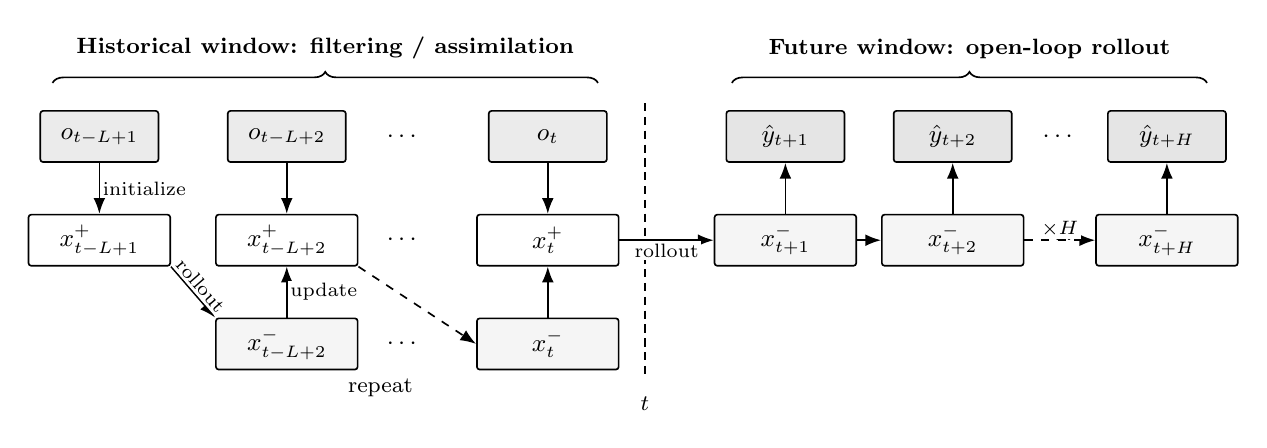
\begin{tikzpicture}[
    x=8.5mm, y=8.5mm,
    >=Latex,
    semithick,
    font=\small,
    obs/.style={
        draw,
        rounded corners=1pt,
        fill=black!8,
        minimum width=15mm,
        minimum height=6.5mm,
        inner sep=1.5pt
    },
    post/.style={
        draw,
        rounded corners=1pt,
        fill=white,
        minimum width=18mm,
        minimum height=6.5mm,
        inner sep=1.5pt
    },
    prior/.style={
        draw,
        rounded corners=1pt,
        fill=black!4,
        minimum width=18mm,
        minimum height=6.5mm,
        inner sep=1.5pt
    },
    pred/.style={
        draw,
        rounded corners=1pt,
        fill=black!10,
        minimum width=15mm,
        minimum height=6.5mm,
        inner sep=1.5pt
    },
    lab/.style={
        font=\scriptsize,
        inner sep=1pt,
        fill=white
    }
]

% =========================================================
% Historical window
% row 1: observations
% row 2: posterior states
% row 3: prior states
% =========================================================
\node[obs]  (o1)  at (0.0,  1.55) {$o_{t-L+1}$};
\node[post] (xp1) at (0.0,  0.00) {$x^{+}_{t-L+1}$};

\node[obs]   (o2)  at (2.8,  1.55) {$o_{t-L+2}$};
\node[post]  (xp2) at (2.8,  0.00) {$x^{+}_{t-L+2}$};
\node[prior] (xm2) at (2.8, -1.55) {$x^{-}_{t-L+2}$};

\node at (4.55,  1.55) {$\cdots$};
\node at (4.55,  0.00) {$\cdots$};
\node at (4.55, -1.55) {$\cdots$};

\node[obs]   (ot)  at (6.70,  1.55) {$o_t$};
\node[post]  (xpt) at (6.70,  0.00) {$x^{+}_{t}$};
\node[prior] (xmt) at (6.70, -1.55) {$x^{-}_{t}$};

% historical arrows
\draw[->] (o1) -- node[right,lab] {initialize} (xp1);

\draw[->] (xp1.south east) --
    node[above,sloped,lab] {rollout}
    (xm2.north west);

\draw[->] (o2) -- (xp2);
\draw[->] (xm2) -- node[right,lab] {update} (xp2);

\draw[->,dashed] (xp2.south east) -- (xmt.west);
\draw[->] (ot) -- (xpt);
\draw[->] (xmt) -- (xpt);

\node[font=\footnotesize] at (4.2,-2.20) {repeat};

% =========================================================
% Separator at time t
% =========================================================
\draw[densely dashed] (8.15,2.05) -- (8.15,-2.05);
\node[font=\footnotesize] at (8.15,-2.45) {$t$};

% =========================================================
% Future window
% row 1: predictions
% row 2: rolled-out latent states
% =========================================================
\node[pred]  (y1)  at (10.25, 1.55) {$\hat y_{t+1}$};
\node[prior] (xf1) at (10.25, 0.00) {$x^{-}_{t+1}$};

\node[pred]  (y2)  at (12.75, 1.55) {$\hat y_{t+2}$};
\node[prior] (xf2) at (12.75, 0.00) {$x^{-}_{t+2}$};

\node at (14.35, 1.55) {$\cdots$};
\node at (14.35, 0.00) {$\cdots$};

\node[pred]  (yH)  at (15.95, 1.55) {$\hat y_{t+H}$};
\node[prior] (xfH) at (15.95, 0.00) {$x^{-}_{t+H}$};

% future arrows
\draw[->] (xpt.east) -- node[below,lab] {rollout} (xf1.west);
\draw[->] (xf1.east) -- (xf2.west);
\draw[->,dashed] (xf2.east) -- node[above,lab] {$\times H$} (xfH.west);

\draw[->] (xf1) -- (y1);
\draw[->] (xf2) -- (y2);
\draw[->] (xfH) -- (yH);

% =========================================================
% Braces / titles
% =========================================================
\draw[decorate,decoration={brace,amplitude=4pt}]
    (-0.70,2.35) -- (7.45,2.35)
    node[midway,above=5pt,font=\footnotesize\bfseries]
    {Historical window: filtering / assimilation};

\draw[decorate,decoration={brace,amplitude=4pt}]
    (9.45,2.35) -- (16.55,2.35)
    node[midway,above=5pt,font=\footnotesize\bfseries]
    {Future window: open-loop rollout};

\end{tikzpicture}
\caption{Inference pipeline of the proposed world-model-based spatiotemporal predictor: filtering / assimilation in the historical window, followed by $H$-step open-loop rollout from the posterior latent state at time $t$.}
\label{fig:inference_pipeline}
\end{figure}

\subsection{记号约定}

\renewcommand{\arraystretch}{1.15}
\noindent
\begin{minipage}[t]{0.66\linewidth}
\raggedright
\begin{tabular}{@{}l@{\hspace{0.8em}}l@{}}
$i\leftarrow j$       & 从节点 $j$ 指向节点 $i$ 的有向边 \\
$x^-$                 & 上标，表示融合当前观测之前的先验状态（prior） \\
$x^+$                 & 上标，表示融合当前观测之后的后验状态（posterior） \\
$x_{\cdot|t}$         & 条件记号，表示“在时刻 $t$ 的已知信息条件下”的估计 \\
$\nu$                 & 在原始观测空间中构造的 innovation 编码 \\
$\hat c^{met}$        & 未来站点级气象摘要（弱监督） \\
$\hat\eta^{src}$      & 未来源机组 latent source summary（默认不做直接监督） \\
$\widetilde{\phi(x)}$ & 再经过训练集统计缩放后的模型输入 \\
$\mathrm{LN}(\cdot)$    & LayerNorm / Layer Normalization / 层归一化 \\
$SiLU$                & Sigmoid Linear Unit \\
\end{tabular}
\end{minipage}\hfill
\begin{minipage}[t]{0.31\linewidth}
\raggedright
\begin{tabular}{@{}l@{\hspace{0.8em}}l@{}}
$q$               & 可用性 mask（有值为 1，无值为 0） \\
$\Delta t$        & 距离最近一次有效观测的时间间隔 \\
$a$               & 动态边 gate / 有向边权重 \\
$e$               & 有向边消息 \\
$m$               & 节点聚合消息 \\
$r$               & 当前观测的 learned representation \\
$\chi$            & 运行状态 / 控制状态指示量 \\
$x$               & 原始物理量 \\
$\phi(x)$         & 物理/几何变换后的量 \\
$\sigma(\cdot)$   & Sigmoid \\
$\odot$           & 逐元素乘法 \\
\end{tabular}
\end{minipage}


\subsection{输入}

本节只定义模型在时刻 $t$ 可直接获得的\textbf{外部输入}。凡是需要结合当前隐状态、编码器或站点聚合后才得到的量，都不再记为“输入”，而在后续小节中单独定义。尤其是 rollout 阶段由模型内部解码得到的未来站点级摘要和未来源机组摘要，属于 latent prediction，而不是已知未来输入。

原始数据中的 companion mask 采用 ``$1$ 表示不可用、$0$ 表示可用'' 的存储约定。为与后续公式保持一致，进入模型前统一转换为
\[
m^{raw}_{k,t}\in\{0,1\},\qquad q_{k,t}=1-m^{raw}_{k,t},
\]
其中 $q_{k,t}=1$ 表示该维当前可用。下文所有网络公式一律使用 $q$，不再直接使用原始 schema 中的 mask 极性。

\subsubsection{节点静态特征}

\begin{equation}
  s_i=\left[\mathrm{Emb}(\mathrm{turbine\_index}_i),\, \widetilde{coord\_x_i},\, \widetilde{coord\_y_i},\, \widetilde{elevation_i},\, \widetilde{rated\_power_i},\, \widetilde{hub\_height_i},\, \widetilde{rotor\_diameter_i}\right]
\end{equation}

\subsubsection{边静态几何特征}

\begin{equation}
  p_{i\leftarrow j}^{stat}=\left[\widetilde{\Delta x_{ij}},\, \widetilde{\Delta y_{ij}},\, \widetilde{\log(1+d_{ij})},\, \widetilde{d^{(RD)}_{ij}},\, \sin(\beta_{ij}),\, \cos(\beta_{ij}),\, \widetilde{\Delta{h}_{ij}} \right]
\end{equation}

\subsubsection{当前机组观测}

记
\[
y^{pu}_{i,t}=\frac{target\_kw_{i,t}}{rated\_power_i},
\]
并用 $ws_{i,t}$、$\omega^{rot}_{i,t}$、$\omega^{gen}_{i,t}$、$T^{amb}_{i,t}$、$T^{nac}_{i,t}$、$\theta^{pitch}_{i,t}$、$wd^{\sin}_{i,t}$、$wd^{\cos}_{i,t}$、$ye^{\sin}_{i,t}$、$ye^{\cos}_{i,t}$ 分别表示风速、主轴转速、发电机转速、环境温度、机舱温度、叶片转角、风向编码和 yaw error 编码。于是
\begin{equation}
  o_{i,t}=\left[
  \begin{aligned}
  &\widetilde{y}^{pu}_{i,t},\, \widetilde{ws}_{i,t},\, \widetilde{\omega}^{rot}_{i,t},\, \widetilde{\omega}^{gen}_{i,t},\, \widetilde{T}^{amb}_{i,t},\, \widetilde{T}^{nac}_{i,t},\, \widetilde{\theta}^{pitch}_{i,t}, \\
  &wd^{\sin}_{i,t},\, wd^{\cos}_{i,t},\, ye^{\sin}_{i,t},\, ye^{\cos}_{i,t}
  \end{aligned}
  \right]
\end{equation}

对应的可用性与 time-gap 记为
\[
q^{obs}_{i,t}\in\{0,1\}^{d_{obs}},\qquad \Delta t^{obs}_{i,t}\ge 0.
\]

\subsubsection{可选的机组运行状态 / 控制输入}

若数据侧可提供运营干预与状态量，则将其作为单独一组输入，而不是与连续观测混在一起。定义
\[
u^{ops}_{i,t}=\left[\chi^{avail}_{i,t},\, \chi^{curt}_{i,t},\, \chi^{fault}_{i,t},\, \chi^{maint}_{i,t},\, \widetilde{p}^{limit,pu}_{i,t},\, \mathrm{emb}(ctrl\_mode_{i,t})\right].
\]

对应的可用性与 time-gap 记为
\[
q^{ops}_{i,t}\in\{0,1\}^{d_{ops}},\qquad \Delta t^{ops}_{i,t}\ge 0.
\]

若部分或全部运行状态信号不可得，则以全零占位，并令相应 mask $q^{ops}_{i,t}=0$。所有实验都应显式记录“是否启用 $u^{ops}$”。

\subsubsection{当前场级可见量}

v1 主模型在当前时刻直接使用的场级外部输入仅包含 PMU 三通道与日历编码。定义
\[
f_t=\left[\widetilde{I}^{farm}_t,\, \widetilde{Q}^{farm}_t,\, \widetilde{P}^{farm}_t\right],\qquad
q^{farm}_t=\left[q^I_t,\, q^Q_t,\, q^P_t\right],
\]
以及
\[
\mathrm{cal}_t=\left[hour^{\sin}_t,\, hour^{\cos}_t,\, weekday^{\sin}_t,\, weekday^{\cos}_t,\, month^{\sin}_t,\, month^{\cos}_t,\, \chi^{weekend}_t\right].
\]

场级事件标记若后续需要启用，可作为 $f_t$ 的附加通道并同步扩展 $q^{farm}_t$；但在 v1 主公式中默认不纳入 $c_t$ 的定义。

\subsubsection{已知未来外生量}

未来时刻唯一允许直接输入模型的外生量仍然只有日历：
\[
u^{known}_{t+\tau}=\mathrm{cal}_{t+\tau},\qquad u^{known}_{i,t+\tau}=\emptyset,\qquad \tau=1,\ldots,H.
\]

\subsection{由当前输入与先验状态构造的中间量}

以下量在时刻 $t$ 由当前输入和 prior state 共同构造，用于 Update / message passing；它们服务于模型内部计算，但不属于外部输入。

\subsubsection{源机组子集与源机组摘要}

先从当前观测中选出与 wake 强度最相关的源机组变量：
\[
x^{src}_{j,t}=\left[\widetilde{y}^{pu}_{j,t},\, \widetilde{ws}_{j,t},\, \widetilde{\theta}^{pitch}_{j,t},\, ye^{\sin}_{j,t},\, ye^{\cos}_{j,t}\right],
\]
并抽取与其最相关的可选运行状态子集
\[
u^{ops,src}_{j,t}=\left[\chi^{avail}_{j,t},\, \chi^{curt}_{j,t},\, \chi^{fault}_{j,t},\, \widetilde{p}^{limit,pu}_{j,t}\right].
\]

对应的子集 mask 与 time-gap 由完整向量投影得到：
\[
q^{src}_{j,t}=\Pi_{src}(q^{obs}_{j,t}),\qquad
q^{ops,src}_{j,t}=\Pi_{ops,src}(q^{ops}_{j,t}),
\]
\[
\Delta t^{src}_{j,t}=\Pi_{src}(\Delta t^{obs}_{j,t}),\qquad
\Delta t^{ops,src}_{j,t}=\Pi_{ops,src}(\Delta t^{ops}_{j,t}).
\]

再通过一个 mask-aware 编码器得到供边网络使用的源机组摘要：
\[
v^{src}_{j,t}=\mathrm{Enc}_{src}\left([x^{src,imp}_{j,t},\, u^{ops,src,imp}_{j,t},\, q^{src}_{j,t},\, q^{ops,src}_{j,t},\, \Delta t^{src}_{j,t},\, \Delta t^{ops,src}_{j,t},\, z^-_{j,t},\, h^-_{j,t},\, s_j]\right).
\]

其中 $x^{src,imp}_{j,t}$ 与 $u^{ops,src,imp}_{j,t}$ 的插补规则与后文 Enc\_obs 小节完全一致。

\subsubsection{Update 阶段的动态边特征}

记当前时刻沿有效风向旋转后的顺风/横风投影距离分别为 $d^{\parallel}_{ij,t}$ 与 $d^{\perp}_{ij,t}$，并以源机组叶轮直径 $D_j$ 做尺度归一化。为避免逆风方向出现指数爆炸，定义平滑的 wake 先验 gate：
\[
\psi^{wake}_{ij,t}=\sigma\!\left(\kappa d^{\parallel}_{ij,t}\right)\cdot \exp\!\left(-\frac{\mathrm{ReLU}(d^{\parallel}_{ij,t})}{\lambda_x}\right)\cdot \exp\!\left(-\left(\frac{d^{\perp}_{ij,t}}{\lambda_y}\right)^2\right).
\]

于是 Update 阶段实际送入边网络的动态特征写为
\[
p^{dyn,upd}_{i\leftarrow j,t}=\left[\frac{d^{\parallel}_{ij,t}}{D_j},\, \frac{d^{\perp}_{ij,t}}{D_j},\, \psi^{wake}_{ij,t},\, v^{src}_{j,t}\right].
\]

\subsubsection{站点级当前上下文}

记 $q^{ws}_{i,t}$ 为风速通道可用标志，$q^{wd}_{i,t}$ 为风向编码成对可用标志；站点级统计只允许使用当前时刻\textbf{真实可用}的节点观测，不使用任何插补值。定义
\[
\bar{ws}_t=\frac{\sum_i q^{ws}_{i,t}\, ws_{i,t}}{\epsilon+\sum_i q^{ws}_{i,t}},\qquad \rho^{ws}_t=\frac{1}{N}\sum_i q^{ws}_{i,t},
\]
\[
C_t=\frac{\sum_i q^{wd}_{i,t}\, wd^{\cos}_{i,t}}{\epsilon+\sum_i q^{wd}_{i,t}},\qquad
S_t=\frac{\sum_i q^{wd}_{i,t}\, wd^{\sin}_{i,t}}{\epsilon+\sum_i q^{wd}_{i,t}},
\]
\[
R_t=\sqrt{C_t^2+S_t^2},\qquad \rho^{wd}_t=\frac{1}{N}\sum_i q^{wd}_{i,t}.
\]

于是当前时刻送入图网络和全局状态更新的站点级上下文为
\[
c_t=\left[\widetilde{\bar{ws}}_t,\, C_t,\, S_t,\, R_t,\, \rho^{ws}_t,\, \rho^{wd}_t,\, f_t,\, q^{farm}_t,\, \mathrm{cal}_t\right].
\]

\subsection{rollout 阶段的模型内部预测量}

以下量仅在未来窗的 Transition 中由模型内部解码得到；它们不是已知未来输入，也不应与 $u^{known}_{t+\tau}$ 混写。

\subsubsection{未来站点级摘要与未来动态图特征}

\[
\hat c^{met}_{t+\tau}=\mathrm{Dec}^{met}_g\left(g_{t+\tau-1|t},\, \mathrm{cal}_{t+\tau}\right),\qquad
\hat c_{t+\tau}=\left[\hat c^{met}_{t+\tau},\, \mathrm{cal}_{t+\tau}\right]
\]
\[
\hat\eta^{src}_{j,t+\tau}=\mathrm{MLP}^{pred}_{src}\left([z_{j,t+\tau-1|t},\, h_{j,t+\tau-1|t},\, s_j,\, g_{t+\tau-1|t}]\right)
\]
\[
\hat p^{dyn,pred}_{i\leftarrow j,t+\tau}=\left[\frac{\hat d^{\parallel}_{ij,t+\tau}}{D_j},\, \frac{\hat d^{\perp}_{ij,t+\tau}}{D_j},\, \hat\psi^{wake}_{ij,t+\tau},\, \hat\eta^{src}_{j,t+\tau}\right].
\]

其中 $\hat d^{\parallel}_{ij,t+\tau}$、$\hat d^{\perp}_{ij,t+\tau}$ 与 $\hat\psi^{wake}_{ij,t+\tau}$ 基于 $\hat c^{met}_{t+\tau}$ 计算得到。语义上，$\hat c^{met}_{t+\tau}$ 被视为\textbf{弱监督的站点级气象摘要}；而 $\hat\eta^{src}_{j,t+\tau}$ 在 v1 中被视为\textbf{仅供边网络使用的 latent source summary}，默认不做逐维直接监督，除非后续实验显式打开 source auxiliary head。

若训练阶段可以从真实未来观测中构造站点级统计量，则定义
\[
c^{met,*}_{t+\tau}=\left[\widetilde{\bar{ws}}_{t+\tau},\, C_{t+\tau},\, S_{t+\tau},\, R_{t+\tau},\, \rho^{ws}_{t+\tau},\, \rho^{wd}_{t+\tau}\right]
\]
并用其作为 $\hat c^{met}_{t+\tau}$ 的弱监督目标；而 $\hat\eta^{src}_{j,t+\tau}$ 只通过 forecast / graph losses 间接训练，默认不引入额外的 pointwise reconstruction loss。

\subsection{结构详情}

\subsubsection{观测编码 Enc\_obs}
Enc\_obs 负责把当前连续观测与本机运行状态联合编码成供图聚合和本机更新使用的节点表示。连续观测沿用 GRU-D 风格的缺失感知输入处理：
$$x_{k,t}^{imp}=q^{obs}_{k,t}x_{k,t}+(1-q^{obs}_{k,t})\left(\gamma^{obs}_{k,t}x_{k,t}^{last}+(1-\gamma^{obs}_{k,t})\bar x_k\right)$$

对离散/控制类运行状态，v1 不做双向插值，而是采用 ``last valid hold + mask/time-gap 显式输入''：
$$u^{ops,imp}_{l,t}=q^{ops}_{l,t}u^{ops}_{l,t}+(1-q^{ops}_{l,t})u^{ops,last}_{l,t}$$

$$\xi^{ops}_{i,t}=\mathrm{LN}\left(\mathrm{MLP}_{ops}\left([u^{ops,imp}_{i,t},\, q^{ops}_{i,t},\, \Delta t^{ops}_{i,t},\, s_i]\right)\right)$$

$$r_{i,t}=\mathrm{LN}\left(\mathrm{MLP}_{obs}\left([x_{i,t}^{imp},\, \xi^{ops}_{i,t},\, q^{obs}_{i,t},\, q^{ops}_{i,t},\, \Delta t^{obs}_{i,t},\, \Delta t^{ops}_{i,t},\, s_i]\right)\right)$$

\noindent 其中 $\Delta t^{obs}_{k,t}$ 是第 $k$ 个连续观测变量距离最近一次有效观测的时间，$\Delta t^{ops}_{l,t}$ 是第 $l$ 个运行状态量距离最近一次有效记录的时间，$q$ 为相应 mask，$\gamma^{obs}_{k,t}$ 为随时间间隔衰减的可信度。这样一来，运营干预不仅会进入源机组摘要 $v^{src}$，也会直接作用于本机观测编码与局部状态更新。需要强调的是：$r_{i,t}$ 只是 learned representation；真正用于 filtering correction 的 innovation 仍在原始观测空间中构造，而不是直接在 $r$ 空间中求差。

\subsubsection{动态图消息传递 $f_{\theta}$、$\Sigma(\varphi)$、$\Sigma(\psi)$}
为同时保留“平均邻居画像”和“累计上游负担”，聚合阶段不再只用加权平均，而是并行提取 sum / mean / mass / max 四个通道。

Update 阶段：
$$e_{i\leftarrow j,t}^{upd}=\mathrm{MLP}_e^{upd}\left([s_i,\, s_j,\, p_{i\leftarrow j}^{stat},\, p_{i\leftarrow j,t}^{dyn,upd},\, g_t^-,\, c_t]\right)$$

$$a_{i\leftarrow j,t}^{upd}=\sigma\left(\mathrm{MLP}_a^{upd}\left([s_i,\, s_j,\, p_{i\leftarrow j}^{stat},\, p_{i\leftarrow j,t}^{dyn,upd},\, g_t^-,\, c_t]\right)\right)$$

$$s_{i,t}^{sum}=\sum_{j\in\mathcal N(i)} a^{upd}_{i\leftarrow j,t}e^{upd}_{i\leftarrow j,t},\qquad s_{i,t}^{mean}=\frac{s_{i,t}^{sum}}{\epsilon+\sum_j a^{upd}_{i\leftarrow j,t}}$$

$$s_{i,t}^{mass}=\sum_{j\in\mathcal N(i)} a^{upd}_{i\leftarrow j,t},\qquad s_{i,t}^{max}=\max_{j\in\mathcal N(i)}\left(a^{upd}_{i\leftarrow j,t}e^{upd}_{i\leftarrow j,t}\right)$$

$$m_{i,t}^{upd}=\mathrm{MLP}^{upd}_{\Sigma}\left([r_{i,t},\, s_{i,t}^{sum},\, s_{i,t}^{mean},\, s_{i,t}^{mass},\, s_{i,t}^{max}]\right)$$

Transition 阶段：
$$e^{pred}_{i\leftarrow j,t+\tau}=\mathrm{MLP}^{pred}_{e}\Big([s_i,\, s_j,\, p^{stat}_{i\leftarrow j},\, \hat p^{dyn,pred}_{i\leftarrow j,t+\tau},\, z_{j,t+\tau-1|t},\, h_{j,t+\tau-1|t},\, g_{t+\tau-1|t},\, \hat c_{t+\tau}]\Big)$$

$$a^{pred}_{i\leftarrow j,t+\tau}=\sigma\Big(\mathrm{MLP}^{pred}_{a}\big([s_i,\, s_j,\, p^{stat}_{i\leftarrow j},\, \hat p^{dyn,pred}_{i\leftarrow j,t+\tau},\, z_{j,t+\tau-1|t},\, h_{j,t+\tau-1|t},\, g_{t+\tau-1|t},\, \hat c_{t+\tau}]\big)\Big)$$

$$\hat s_{i,t+\tau}^{sum}=\sum_{j\in\mathcal N(i)} a^{pred}_{i\leftarrow j,t+\tau}e^{pred}_{i\leftarrow j,t+\tau},\qquad \hat s_{i,t+\tau}^{mean}=\frac{\hat s_{i,t+\tau}^{sum}}{\epsilon+\sum_j a^{pred}_{i\leftarrow j,t+\tau}}$$

$$\hat s_{i,t+\tau}^{mass}=\sum_{j\in\mathcal N(i)} a^{pred}_{i\leftarrow j,t+\tau},\qquad \hat s_{i,t+\tau}^{max}=\max_{j\in\mathcal N(i)}\left(a^{pred}_{i\leftarrow j,t+\tau}e^{pred}_{i\leftarrow j,t+\tau}\right)$$

$$m^{pred}_{i,t+\tau}=\mathrm{MLP}^{pred}_{\Sigma}\left([\hat s_{i,t+\tau}^{sum},\, \hat s_{i,t+\tau}^{mean},\, \hat s_{i,t+\tau}^{mass},\, \hat s_{i,t+\tau}^{max}]\right)$$

\subsubsection{图构造与邻域更新的最终约定}
v1 将用于几何旋转的风向固定为站点级 masked circular mean：
$$\theta^{site}_t=\mathrm{atan2}(S_t,\, C_t),\qquad \hat\theta^{site}_{t+\tau}=\mathrm{atan2}(\hat S_{t+\tau},\, \hat C_{t+\tau})$$
历史窗与未来窗都按该角度对 $(\Delta x,\Delta y)$ 做旋转，得到 $d^{\parallel}$ 与 $d^{\perp}$。为避免每步在全图上重新搜边，v1 先依据静态几何构造一个\textbf{固定候选池}：
$$\mathcal E^{cand}(i)=\left\{j\neq i\;\middle|\; d^{(RD)}_{ij}\le r_{cand}\right\},\qquad r_{cand}=25.$$
每个时间步只在 $\mathcal E^{cand}(i)$ 内更新 $d^{\parallel}$、$d^{\perp}$、$\psi^{wake}$ 与动态边特征，并按 wake gate 取物理 top-$K$：
$$\mathcal N^{phys}_t(i)=\mathrm{TopK}_{j\in \mathcal E^{cand}(i)}\left(\psi^{wake}_{ij,t},\, K\right),\qquad K=8\sim 12.$$

为补充纯几何图无法覆盖的非局地相关性，再引入少量 learned residual edges。其打分由节点嵌入形成的低秩自适应得分给出：
$$a^{res}_{i\leftarrow j}=\frac{\xi_i^\top \xi_j}{\sqrt{d_{res}}},\qquad \mathcal E^{res}(i)=\mathrm{TopK}_{j\notin \mathcal E^{cand}(i)}\left(a^{res}_{i\leftarrow j},\, K_{res}\right).$$
最终邻域定义为
$$\mathcal N_t(i)=\mathcal N^{phys}_t(i)\cup \mathcal E^{res}(i).$$

\noindent v1 默认\textbf{不保留 self-loop}，因为节点自身的信息已经通过 $r_i$、$z_i$、$h_i$ 与 $s_i$ 直接输入 Update / Transition；若同时加入 self-loop，往往会形成重复计数。

\subsubsection{历史窗口中的 prior propagation 与 filtering 闭环}
历史窗口中的状态闭环按 ``\textbf{先 Transition 得到 prior，再用真实观测做 Update}'' 执行。为避免训练/推理阶段出现两套不同的状态机，v1 默认\textbf{共享} rollout 阶段的 Transition / Transition$_g$ 参数来完成历史窗的 prior 传播，而不是另外再写一套 history-only dynamics。给定上一时刻后验
$$\left\{z^+_{i,t-1},\, h^+_{i,t-1}\right\}_{i=1}^N,\qquad g^+_{t-1},$$
先由上一时刻后验状态解码当前时刻的先验上下文：
$$\hat c^{met}_{t|t-1}=\mathrm{Dec}^{met}_g\left(g^+_{t-1},\, \mathrm{cal}_{t}\right),\qquad \bar c_{t|t-1}=\left[\hat c^{met}_{t|t-1},\, \mathrm{cal}_{t}\right]$$
$$\hat\eta^{src}_{j,t|t-1}=\mathrm{MLP}^{pred}_{src}\left([z^+_{j,t-1},\, h^+_{j,t-1},\, s_j,\, g^+_{t-1}]\right)$$
$$\hat p^{dyn,pred}_{i\leftarrow j,t|t-1}=\left[\frac{\hat d^{\parallel}_{ij,t|t-1}}{D_j},\, \frac{\hat d^{\perp}_{ij,t|t-1}}{D_j},\, \hat\psi^{wake}_{ij,t|t-1},\, \hat\eta^{src}_{j,t|t-1}\right].$$
随后在当前时刻的候选邻域 $\mathcal N_t(i)$ 内计算先验图消息：
$$m^{pred}_{i,t|t-1}=\Sigma^{pred}\left(\left\{e^{pred}_{i\leftarrow j,t|t-1}\right\}_{j\in \mathcal N_t(i)}\right).$$
并用与 rollout 完全相同的局部/全局转移接口完成一步 prior propagation：
$$\left(z^-_{i,t},\, h^-_{i,t}\right)=\mathrm{Transition}\left(z^+_{i,t-1},\, h^+_{i,t-1},\, m^{pred}_{i,t|t-1},\, g^+_{t-1},\, \bar c_{t|t-1},\, s_i\right)$$
$$\bar n^{tr}_{t|t-1}=\mathrm{Pool}^{tr}\left(\{z^+_{i,t-1},\, h^+_{i,t-1},\, s_i\}_{i=1}^N\right),\qquad g^-_{t}=\mathrm{Transition}_g\left(g^+_{t-1},\, \bar n^{tr}_{t|t-1},\, \bar c_{t|t-1}\right).$$
最后再用真实观测执行 posterior correction。这里将局部更新与全局更新显式拆开，以消除 Update / Update$_g$ 接口歧义：
$$\left\{z^+_{i,t},\, h^+_{i,t}\right\}_{i=1}^N=\mathrm{Update}\left(\left\{z^-_{i,t},\, h^-_{i,t}\right\}_{i=1}^N,\, g^-_t,\, \left\{o_{i,t}\right\}_{i=1}^N,\, \left\{\xi^{ops}_{i,t}\right\}_{i=1}^N,\, c_t,\, \left\{s_i\right\}_{i=1}^N\right)$$
$$\bar n^+_{t}=\mathrm{Pool}^{+}\left(\{z^+_{i,t},\, h^+_{i,t},\, s_i,\, \rho^{node}_{i,t}\}_{i=1}^N\right),\qquad g^+_{t}=\mathrm{Update}_g\left(g^-_t,\, \bar n^+_t,\, c_t\right).$$
这样历史窗、验证推理与测试推理使用的是同一套 local/global state machine，只是历史窗在每步 prior 传播之后还会再接入真实观测做一次 posterior correction。

\subsubsection{初始化与长缺测处理}
v1 将每个样本窗口的首个时刻记为 $t_0$。初始后验状态由静态特征唯一决定：
$$z^+_{i,t_0-1}=W^{init}_z s_i,\qquad h^+_{i,t_0-1}=W^{init}_h s_i$$
$$g^+_{t_0-1}=W^{init}_g\left(\frac{1}{N}\sum_{i=1}^{N}\mathrm{MLP}^{init}_g(s_i)\right).$$
当首个时间步不存在最近一次有效观测时，固定采用以下初始化规则：
$$x^{last}_{k,t_0-1}=\bar x_k,\qquad u^{ops,last}_{l,t_0-1}=0,\qquad q^{obs,last}_{k,t_0-1}=0,\qquad q^{ops,last}_{l,t_0-1}=0$$
$$\Delta t^{obs}_{k,t_0}=\Delta t^{ops}_{l,t_0}=\Delta t_{max},\qquad \Delta t_{max}=72\Delta=720\,\mathrm{min}. $$
若某台机组在样本窗口中连续 $G_{gap}=36$ 个时间步（即 $6$ 小时）以上对关键局部观测子集 $\{y^{pu},ws,rotor\_rpm,gen\_rpm,pitch\}$ 全部缺失，则对应时间段内停止本机 Update，仅保留 Transition 传播，并强制其池化权重 $\omega^{pool}_{i,t}=0$。若该关键子集在整个 $144$ 步历史窗口内均缺失，则该 turbine-window 不参与 $L_{hist\_recon}$ 与 $L_{forecast}$ 的局部项，只保留其对场级约束的占位影响。

\subsubsection{隐状态的更新与转移}
Update 阶段的 innovation 在原始观测空间中构造，而不是在 $r$ 空间中直接做差。先用 prior state 预测当前观测：
$$\hat o^-_{i,t}=\mathrm{Dec}_{obs}\left([z^-_{i,t},\, h^-_{i,t},\, g_t^-,\, s_i]\right)$$

再构造 masked residual：
$$\delta o_{i,t}=q^{obs}_{i,t}\odot\left(o_{i,t}-\hat o^-_{i,t}\right)$$

并将其编码成 innovation：
$$\nu_{i,t}=\mathrm{Enc}_{\nu}\left([\hat o^-_{i,t},\, \delta o_{i,t},\, q^{obs}_{i,t},\, \Delta t^{obs}_{i,t},\, r_{i,t},\, \xi^{ops}_{i,t}]\right)$$

\noindent 其中 $r_{i,t}$ 只作为辅助表征输入，不再作为 innovation 的主语义坐标系；$\xi^{ops}_{i,t}$ 则确保运营干预会直接进入本机更新路径。

对于快变量：
$$q_{i,t}^z=\left[z_{i,t}^-,\, \nu_{i,t},\, \xi^{ops}_{i,t},\, m_{i,t}^{upd},\, g_t^-,\, c_t,\, s_i\right]$$

$$\rho_{i,t}^z=\sigma\left(W_r^zq_{i,t}^z+b_r^z\right)$$

$$\tilde z_{i,t}^{upd}=\tanh\left(W_h^z\left[\rho_{i,t}^z\odot z_{i,t}^-,\, \nu_{i,t},\, \xi^{ops}_{i,t},\, m_{i,t}^{upd},\, g_t^-,\, c_t,\, s_i\right]+b_h^z\right)$$

$$\alpha_{i,t}^z=\sigma\left(W_\alpha^zq_{i,t}^z+b_\alpha^z\right)$$

$$z_{i,t}^+=(1-\alpha_{i,t}^z)\odot z_{i,t}^-+\alpha_{i,t}^z\odot \tilde z_{i,t}^{upd}$$

对于慢变量：
$$\bar \nu_{i,t}=\mathrm{MLP}_{lp}\left([\nu_{i,t},\, \xi^{ops}_{i,t},\, m_{i,t}^{upd},\, z_{i,t}^+-z_{i,t}^-]\right)$$

$$q_{i,t}^h=\left[h_{i,t}^-,\, z_{i,t}^+,\, \bar \nu_{i,t},\, \xi^{ops}_{i,t},\, m_{i,t}^{upd},\, g_t^-,\, c_t,\, s_i\right]$$

$$\rho_{i,t}^h=\sigma\left(W_r^hq_{i,t}^h+b_r^h\right)$$

$$\tilde h_{i,t}^{upd}=\tanh\left(W_h^h\left[\rho_{i,t}^h\odot h_{i,t}^-,\, z_{i,t}^+,\, \bar \nu_{i,t},\, \xi^{ops}_{i,t},\, m_{i,t}^{upd},\, g_t^-,\, c_t,\, s_i\right]+b_h^h\right)$$

$$\alpha_{i,t}^h=\alpha^{h,max}\cdot \sigma\left(W_\alpha^hq_{i,t}^h+b_\alpha^h\right),\qquad \alpha^{h,max}\in [0.05,0.2]$$

$$h_{i,t}^+=(1-\alpha_{i,t}^h)\odot h_{i,t}^-+\alpha_{i,t}^h\odot \tilde h_{i,t}^{upd}$$

Transition 阶段：
$$q^{z,tr}_{i,t+\tau}=\left[z_{i,t+\tau-1|t},\, h_{i,t+\tau-1|t},\, m^{pred}_{i,t+\tau},\, g_{t+\tau-1|t},\, \hat c_{t+\tau},\, s_i\right]$$

$$\rho^{z,tr}_{i,t+\tau}=\sigma\left(W^{z,tr}_{r}q^{z,tr}_{i,t+\tau}+b^{z,tr}_{r}\right)$$

$$\tilde z^{tr}_{i,t+\tau}=\tanh\Big(W^{z,tr}_{h}\big[\rho^{z,tr}_{i,t+\tau}\odot z_{i,t+\tau-1|t},\, h_{i,t+\tau-1|t},\, m^{pred}_{i,t+\tau},\, g_{t+\tau-1|t},\, \hat c_{t+\tau},\, s_i\big]+b^{z,tr}_{h}\Big)$$

$$\beta^{z}_{i,t+\tau}=\sigma\left(W^{z,tr}_{\beta}q^{z,tr}_{i,t+\tau}+b^{z,tr}_{\beta}\right)$$

$$z_{i,t+\tau|t}=(1-\beta^{z}_{i,t+\tau})\odot z_{i,t+\tau-1|t}+\beta^{z}_{i,t+\tau}\odot \tilde z^{tr}_{i,t+\tau}$$

$$q^{h,tr}_{i,t+\tau}=\left[h_{i,t+\tau-1|t},\, z_{i,t+\tau|t},\, m^{pred}_{i,t+\tau},\, g_{t+\tau-1|t},\, \hat c_{t+\tau},\, s_i\right]$$

$$\tilde h^{tr}_{i,t+\tau}=\tanh\Big(W^{h,tr}_{2}\, \mathrm{SiLU}(W^{h,tr}_{1}q^{h,tr}_{i,t+\tau})\Big)$$

$$\beta^{h}_{i,t+\tau}=\beta^{h,\max}\cdot \sigma\left(W^{h,tr}_{\beta}q^{h,tr}_{i,t+\tau}+b^{h,tr}_{\beta}\right),\qquad \beta^{h,\max}\in[0.05,0.15]$$

$$h_{i,t+\tau|t}=(1-\beta^{h}_{i,t+\tau})\odot h_{i,t+\tau-1|t}+\beta^{h}_{i,t+\tau}\odot \tilde h^{tr}_{i,t+\tau}$$

\subsubsection{全局状态 Update\_g / Transition\_g}
为避免实现者写出两套不同的 global dynamics，v1 明确固定两个接口：
$$g_t^+=\mathrm{Update}_g\left(g_t^-,\, \bar n_t^+,\, c_t\right),\qquad g' = \mathrm{Transition}_g\left(g,\, \bar n^{tr},\, \bar c\right).$$
其中 Update$_g$ 只在历史窗的 posterior correction 之后调用；Transition$_g$ 同时用于历史窗 prior propagation 和未来 rollout，输入签名在两种场景下保持完全一致。

先定义节点级可用率
$$\rho^{node}_{i,t}=\frac{1}{d_{obs}}\sum_{k=1}^{d_{obs}} q^{obs}_{i,t,k}$$
以及 posterior pooling 所需的节点摘要
$$u^{pool,+}_{i,t}=\mathrm{MLP}^{+}_{pool}\left([h_i^+,\, z_i^+,\, s_i,\, \rho^{node}_{i,t}]\right).$$

再用一个依赖可用率的 gate 进行集合池化：
$$\omega^{pool,+}_{i,t}=\sigma\left(\mathrm{MLP}^{a,+}_{pool}\left([u^{pool,+}_{i,t},\, \rho^{node}_{i,t},\, s_i]\right)\right),\qquad \bar n^+_t=\frac{\sum_i \omega^{pool,+}_{i,t}u^{pool,+}_{i,t}}{\epsilon+\sum_i \omega^{pool,+}_{i,t}}$$

$$g_t^+=\mathrm{Update}_g\left(g_t^-,\, \bar n^+_t,\, c_t\right).$$

在 prior propagation / rollout 阶段，先从上一时刻全局状态解码未来站点级气象摘要，再用其参与动态图构造：
$$\hat c^{met}_{t+\tau}=\mathrm{Dec}^{met}_g\left(g_{t+\tau-1|t},\, \mathrm{cal}_{t+\tau}\right),\qquad \hat c_{t+\tau}=\left[\hat c^{met}_{t+\tau},\, \mathrm{cal}_{t+\tau}\right]$$

并定义统一的 prior/rollout pooling：
$$u^{pool,tr}_{i,t+\tau}=\mathrm{MLP}^{tr}_{pool}\left([h_{i,t+\tau|t},\, z_{i,t+\tau|t},\, s_i]\right),\qquad \omega^{pool,tr}_{i,t+\tau}=\sigma\left(\mathrm{MLP}^{a,tr}_{pool}\left([u^{pool,tr}_{i,t+\tau},\, s_i]\right)\right)$$

$$\bar n^{tr}_{t+\tau}=\frac{\sum_i \omega^{pool,tr}_{i,t+\tau}u^{pool,tr}_{i,t+\tau}}{\epsilon+\sum_i \omega^{pool,tr}_{i,t+\tau}},\qquad g_{t+\tau|t}=\mathrm{Transition}_g\left(g_{t+\tau-1|t},\, \bar n^{tr}_{t+\tau},\, \hat c_{t+\tau}\right).$$

\subsubsection{Decode 与输出约束}
先由局部/全局隐状态产生未约束输出：
$$\hat y^{raw}_{i,t+\tau|t}=\mathrm{MLP}^{raw}_{dec}\left([h_{i,t+\tau|t},\, z_{i,t+\tau|t},\, g_{t+\tau|t},\, \mathrm{emb}(\tau),\, s_i]\right)$$
再通过有界映射得到 per-unit 功率预测：
$$\hat y^{pu}_{i,t+\tau|t}=(1+\epsilon_y)\,\sigma\left(\hat y^{raw}_{i,t+\tau|t}\right),\qquad \epsilon_y=0.05.$$

\noindent 训练与推理都直接使用该有界输出头，不再额外对预测值做后处理 clip；这样单机输出天然落在 $[0,1+\epsilon_y]$ 范围内，既避免负功率，也允许少量超额定冗余来吸收测量与标定误差。

场级一致性头采用一个可学习的仿射校正：
$$\hat P^{farm}_{t+\tau|t}=b_0+b_1\sum_{i=1}^N rated\_power_i\cdot \hat y^{pu}_{i,t+\tau|t},\qquad b_0\leftarrow 0,\; b_1\leftarrow 1.$$

\noindent 其中 $b_0,b_1$ 为可学习标量，用于吸收线路损耗、PMU 标定偏差与 turbine-sum 到 farm-level power 之间的固定偏移。若后续实验确认还有额外收益，可再叠加独立的场级 auxiliary head；但 v1 默认只启用上述仿射一致性头，以减少实现歧义。
\subsection{可直接启动的超参数与训练策略}

基于当前网络结构，一个可直接启动且实现风险较低的配置如下。整体上，模型容量应优先控制在“足以表达局部时空交互，但不过早引入过强自由度”的范围内，以便先验证动态图建模与全局状态建模是否能够稳定带来收益。在固定单风场设定下，可保留 turbine id embedding；若目标是跨风场泛化，则更建议直接移除该项，以避免模型对风机身份索引产生过强依赖。局部状态采用 \(z/h\) 双变量形式，其中 \(z\) 用于刻画相对快速变化的局部隐变量，\(h\) 用于承载相对平滑的记忆状态；全场摘要状态 \(g\) 则用于建模跨机组的全局背景与场级约束。推荐的启动超参数见表~\ref{tab:hyperparams_startup}。

\begin{table}[!ht]
\centering
\caption{建议的启动超参数配置}
\label{tab:hyperparams_startup}
\renewcommand{\arraystretch}{1.15}
\begin{tabularx}{0.96\linewidth}{@{}lX@{}}
\hline
\textbf{模块/项目}                     & \textbf{推荐设置}                                                                 \\
\hline
Turbine ID embedding                   & 8（仅固定风场时使用；跨风场泛化时建议移除）                                       \\
Static encoder 输出维度                & 32                                                                                \\
Observation encoder 输出 \(r\)         & 64                                                                                \\
Source summary \(v^{src}\)             & 32                                                                                \\
Innovation encoder 输出 \(\nu\)        & 32                                                                                \\
可选运行状态输入 $u^{ops}$            & 若存在则建议压缩到 8\(\sim\)16 维；否则用零向量和 mask 占位                               \\
Edge message 维度                      & 64                                                                                \\
局部隐状态 \(z\)                       & 32                                                                                \\
局部记忆状态 \(h\)                     & 64                                                                                \\
全局状态 \(g\)                         & 48                                                                                \\
Horizon embedding                      & 16                                                                                \\
$\mathrm{MLP}^{upd}_{\Sigma}$ / $\mathrm{MLP}^{pred}_{\Sigma}$ hidden & 128                                     \\
$\alpha^{h,max}$                       & 0.1                                                                               \\
$\beta^{h,max}$                        & 0.1                                                                               \\
Wake prior \(\lambda_x\)              & 4\(\sim\)8（顺风衰减尺度，建议以 rotor-diameter 归一化后调参）                    \\
Wake prior \(\lambda_y\)              & 1.5\(\sim\)3（横风衰减尺度）                                                      \\
Wake gate 斜率 \(\kappa\)             & 1\(\sim\)3                                                                       \\
每时间步 message passing 层数          & 1；最多不超过 2                                                                    \\
候选邻居数                             & 先用静态几何构造候选池 \(d^{(RD)}\le 25\)，再在候选池内按 wake gate 取 top-\(K=8\sim12\) \\
Learned residual edges                 & 2\(\sim\)4 条；仅在候选池外由低秩自适应得分 $a^{res}_{i\leftarrow j}$ 选出           \\
输出上界 $\epsilon_y$                 & 0.05（若数据中存在稳定过额定发电，可上调）                                             \\
Activation                             & SiLU                                                                              \\
Normalization                          & LayerNorm                                                                         \\
Dropout                                & 0.05；通常不建议超过 0.1                                                          \\
Optimizer                              & AdamW                                                                             \\
Learning rate                          & \(2\times 10^{-4}\)                                                               \\
Weight decay                           & \(10^{-4}\)                                                                       \\
Gradient clipping                      & 1.0                                                                               \\
Mixed precision                        & 开启                                                                              \\
Batch size                             & 按序列窗口数计，通常从 8\(\sim\)32 个窗口起步                                     \\
\hline
\end{tabularx}
\end{table}

若第一版实现希望进一步降低结构复杂度，也可采用更保守的替代方案：将 \(z\) 与 \(h\) 合并为一个 64 维的 local state，优先验证动态图与 global state 的增益；待基线结果稳定后，再恢复为快慢变量解耦的双状态形式。这样的简化能够减少训练不稳定性，也更有利于快速确认结构设计中的主要收益来源。

训练方面，最关键的原则是：\textbf{未来时段的 rollout 必须按照推理阶段的开环方式进行训练}。换言之，模型在训练时就应暴露于与测试阶段一致的状态传播路径，而不能仅依赖逐步使用真实未来观测的“教师强制”式训练。基于这一原则，本文建议采用三阶段训练流程，如表~\ref{tab:training_stages} 所示。

\begin{table}[!ht]
\centering
\caption{建议的三阶段训练流程}
\label{tab:training_stages}
\renewcommand{\arraystretch}{1.15}
\begin{tabularx}{0.96\linewidth}{@{}lX@{}}
\hline
\textbf{阶段} & \textbf{训练目标与设置} \\
\hline
阶段 A：短 horizon 预训练 &
使用较短 rollout（如 6 或 12 步）联合训练 \(\mathrm{Enc}_{\mathrm{obs}}\)、Update、Transition 与 Decode。损失以历史末端的当前/一步预测和少量未来 rollout loss 为主。该阶段的目标不是获得最终精度，而是先将 filter/update 过程训练稳定。 \\
\hline
阶段 B：全长训练 &
对每个样本使用完整的 \(144\) 步 lookback 与 \(36\) 步未来 rollout。历史部分可划分为两段：前 \(72\sim108\) 步作为 burn-in，仅用于更新状态，不反传或仅施加较弱重建损失；后 \(36\sim72\) 步用于施加原始观测空间 reconstruction / consistency loss；未来 \(36\) 步施加主 forecast loss。该策略可显著降低显存压力，并更符合“利用历史窗口预热隐状态”的设计目的。 \\
\hline
阶段 C：鲁棒性训练 &
在正式配置上加入三类扰动增强：随机 sensor dropout、随机 edge dropout，以及对风速、温度、转速（RPM）等连续变量施加小幅噪声扰动。这样做的目的是提升模型对真实 SCADA/PMU 数据中坏点、抖动与缺测现象的鲁棒性，减轻其在 latent space 中引发的状态漂移。 \\
\hline
\end{tabularx}
\end{table}

v1 将所有\textbf{连续回归头}统一固定为 Huber loss；二值状态位只作为输入，不在 v1 中单独监督。记
\[
\mathrm{Huber}_{\delta}(u)=
\begin{cases}
\frac{1}{2}u^2/\delta, & |u|\le \delta,\\
|u|-\frac{1}{2}\delta, & |u|>\delta.
\end{cases}
\]
在默认的 $L=144$、$H=36$、$\Delta=10\,\mathrm{min}$ 配置下，固定 burn-in 长度 $L_{burn}=108$，因此历史重建只作用于最后 $36$ 个历史时间步：
\[
\mathcal T_{hist}^{loss}=\{t_0+108,\ldots,t_0+143\},\qquad w_\tau=\frac{1}{H},\ \tau=1,\ldots,H.
\]
其中 $w_\tau$ 为未来 horizon 的固定均匀权重，v1 不再保留“是否加权”的自由度。

首先定义主预测损失：
\[
L_{\mathrm{forecast}}
=
\frac{1}{NH}\sum_{i=1}^{N}\sum_{\tau=1}^{H} q^{y}_{i,t+\tau}\,w_\tau\,\mathrm{Huber}_{\delta_y}\!\left(\hat y^{pu}_{i,t+\tau|t}-y^{pu}_{i,t+\tau}\right),
\qquad \delta_y=0.03.
\]

再定义 posterior decode：
\[
\hat o^+_{i,t}=\mathrm{Dec}^{post}_{obs}\left([z^+_{i,t},\, h^+_{i,t},\, g_t^+,\, s_i]\right).
\]
于是历史重建损失固定为
\[
\begin{aligned}
L_{\mathrm{hist\_recon}}
&=
\frac{1}{N|\mathcal T_{hist}^{loss}|}
\sum_{t\in \mathcal T_{hist}^{loss}}\sum_{i=1}^{N}
\Big(
0.25\,\mathrm{Huber}_{\delta_o}\big(q^{obs}_{i,t}\odot(\hat o^-_{i,t}-o_{i,t})\big)\\
&\hspace{3.8cm}+
0.75\,\mathrm{Huber}_{\delta_o}\big(q^{obs}_{i,t}\odot(\hat o^+_{i,t}-o_{i,t})\big)
\Big),
\qquad \delta_o=0.05.
\end{aligned}
\]

场级一致性损失固定在 farm per-unit 口径上定义。记
\[
y^{farm,pu}_{t}=\frac{P^{farm}_{t}}{\sum_i rated\_power_i},
\qquad
\hat y^{farm,pu}_{t+\tau|t}=\frac{\hat P^{farm}_{t+\tau|t}}{\sum_i rated\_power_i},
\]
则
\[
L_{\mathrm{farm}}
=
\frac{1}{H}\sum_{\tau=1}^{H}
\mathrm{Huber}_{\delta_f}\left(\hat y^{farm,pu}_{t+\tau|t}-y^{farm,pu}_{t+\tau}\right),
\qquad \delta_f=0.03.
\]

为避免 ``$\hat c^{met}$ 被赋予物理名字但训练上毫无约束''，v1 额外引入一个弱监督的站点级气象摘要损失。将
\[
\hat c^{met}_{t+\tau}=
\left[\widehat{\bar{ws}}_{t+\tau},\, \hat C_{t+\tau},\, \hat S_{t+\tau},\, \hat R_{t+\tau},\, \hat\rho^{ws}_{t+\tau},\, \hat\rho^{wd}_{t+\tau}\right]
\]
与真实未来统计量
\[
c^{met,*}_{t+\tau}=
\left[\bar{ws}_{t+\tau},\, C_{t+\tau},\, S_{t+\tau},\, R_{t+\tau},\, \rho^{ws}_{t+\tau},\, \rho^{wd}_{t+\tau}\right]
\]
对齐，定义
\[
\begin{aligned}
L_{\mathrm{met}}
&=
\frac{1}{H}\sum_{\tau=1}^{H}
\Big(
\mathrm{Huber}_{0.05}(\widehat{\bar{ws}}_{t+\tau}-\bar{ws}_{t+\tau})
+0.5\,\|\hat C_{t+\tau}-C_{t+\tau}\|_2^2
+0.5\,\|\hat S_{t+\tau}-S_{t+\tau}\|_2^2 \\
&\hspace{2.2cm}+
0.25\,\mathrm{Huber}_{0.05}(\hat R_{t+\tau}-R_{t+\tau})
+0.25\,\mathrm{Huber}_{0.05}(\hat\rho^{ws}_{t+\tau}-\rho^{ws}_{t+\tau})
+0.25\,\mathrm{Huber}_{0.05}(\hat\rho^{wd}_{t+\tau}-\rho^{wd}_{t+\tau})
\Big).
\end{aligned}
\]
$\hat\eta^{src}$ 在 v1 中仍被视为 latent source summary，默认不加入逐维直接监督，因此固定取 $\lambda_{src}=0$，不启用 $L_{src}^{opt}$。

Innovation 正则项也在 v1 中定版为
\[
L_{\mathrm{innovation}}
=
\frac{1}{N|\mathcal T_{hist}^{loss}|}
\sum_{t\in \mathcal T_{hist}^{loss}}\sum_{i=1}^{N}
\left(
\frac{\|z^+_{i,t}-z^-_{i,t}\|_2^2}{d_z}
+
0.5\,\frac{\|h^+_{i,t}-h^-_{i,t}\|_2^2}{d_h}
\right)
+
0.25\,\frac{1}{|\mathcal T_{hist}^{loss}|}
\sum_{t\in \mathcal T_{hist}^{loss}}
\frac{\|g_t^+-g_t^-\|_2^2}{d_g}.
\]

综合考虑预测精度、状态一致性、场级约束与未来站点摘要监督，v1 的最终训练目标固定为
\[
L
=
1.0\,L_{\mathrm{forecast}}
+0.2\,L_{\mathrm{hist\_recon}}
+0.1\,L_{\mathrm{farm}}
+0.05\,L_{\mathrm{met}}
+10^{-4}L_{\mathrm{innovation}}.
\]

此外，v1 默认\textbf{不将}上一时刻预测值 $\hat{y}_{t+\tau-1|t}$ 回灌给下一时刻 Transition 输入；Transition 只在 latent space 中运行。因此 scheduled sampling 在本版本中固定关闭，不作为标准训练组件。只有当后续实验显式改成基于输出回灌的自回归解码器时，才再考虑引入 scheduled sampling。

\subsection{评估与消融协议}
为形成完整的研究闭环，v1 在首轮实验中固定如下评估协议：
\begin{itemize}
  \item \textbf{切分方式：}仅允许按时间连续块切分 train / validation / test，禁止随机打散；若数据覆盖多个季节，至少额外报告一次 rolling-origin 的跨季节回测结果。
  \item \textbf{主指标：}报告 turbine-level 与 farm-level 两组指标，至少包含 MAE、RMSE；同时给出 per-unit 口径与 kW 口径；对未来 $36$ 步逐 horizon 报告，并汇总成短期（1--12 步）、中期（13--24 步）、长期（25--36 步）三档结果。
  \item \textbf{分组评估：}按风向扇区、可用率高低、正常工况/限电工况（若有标签）分别汇报，避免单一平均指标掩盖关键工况退化。
  \item \textbf{内部基线与消融：}至少包含 persistence / last-value baseline、无动态图版本、无 global state 版本、单状态（以单个 local state 替代 $z+h$）版本；同时比较去掉 $u^{ops}$、去掉 $L_{met}$、去掉 learned residual edges、去掉 PMU、将输出头从有界形式改为无界线性头等开关。
\end{itemize}

\paragraph{强非图神经基线（固定）}
为严格评估动态图的净收益，v1 额外固定一个强的非图神经基线：\textbf{shared-weight TFT-no-graph}。该基线以每台机组为一个样本实例，输入同一套历史局部观测 $o_{i,t-L+1:t}$、可选运行状态 $u^{ops}_{i,t-L+1:t}$、静态属性 $s_i$、站点级上下文 $c_{t-L+1:t}$ 与已知未来日历 $\mathrm{cal}_{t+1:t+H}$，但\textbf{不使用任何图边、邻机消息传递、局部/全局 latent state 分解或显式的 farm global state}。模型参数在所有机组间共享，训练窗口、数据切分、早停规则和主预测损失与主模型保持一致。这样在结果表中可以直接比较 ``shared covariate model'' 与 ``wake-aware dynamic graph model'' 之间的差异。

\paragraph{复现实验规范（固定）}
设全数据按时间排序后共有 $M$ 个统一时间步，默认固定连续切分边界为
\[
b_1=\lfloor 0.70M \rfloor,
\qquad
b_2=\lfloor 0.85M \rfloor,
\qquad
G=L+H=180\ \mathrm{steps}=30\ \mathrm{hours}.
\]
则训练集、验证集、测试集分别为
\[
\mathcal D_{train}=[1,b_1],\qquad
\mathcal D_{val}=[b_1+G+1,b_2],\qquad
\mathcal D_{test}=[b_2+G+1,M].
\]
这里预留的 $G=180$ 步 gap 用于切断 lookback 与 forecast horizon 对跨边界样本的感受野泄漏。所有缩放统计量、异常阈值统计和可学习初始化参数只能用 $\mathcal D_{train}$ 估计。

随机种子固定为 $\{3407,3408,3409\}$ 三个独立运行；主表汇报三次运行的均值 $\pm$ 标准差。Early stopping 指标固定为验证集上的 turbine-level MAE（对全部 horizon 均匀平均），patience 固定为 $10$ 个 epoch。Checkpoint 选择规则固定为：首先选验证 MAE 最低者；若差异小于 $10^{-4}$，则选验证 farm-level MAE 更低者；若仍并列，则取更早的 epoch。除非特别说明，所有对比模型都使用同一组切分、同一组随机种子和同一套 checkpoint 选择规则。

\subsection{示意图}

\begin{figure}[t]
\centering
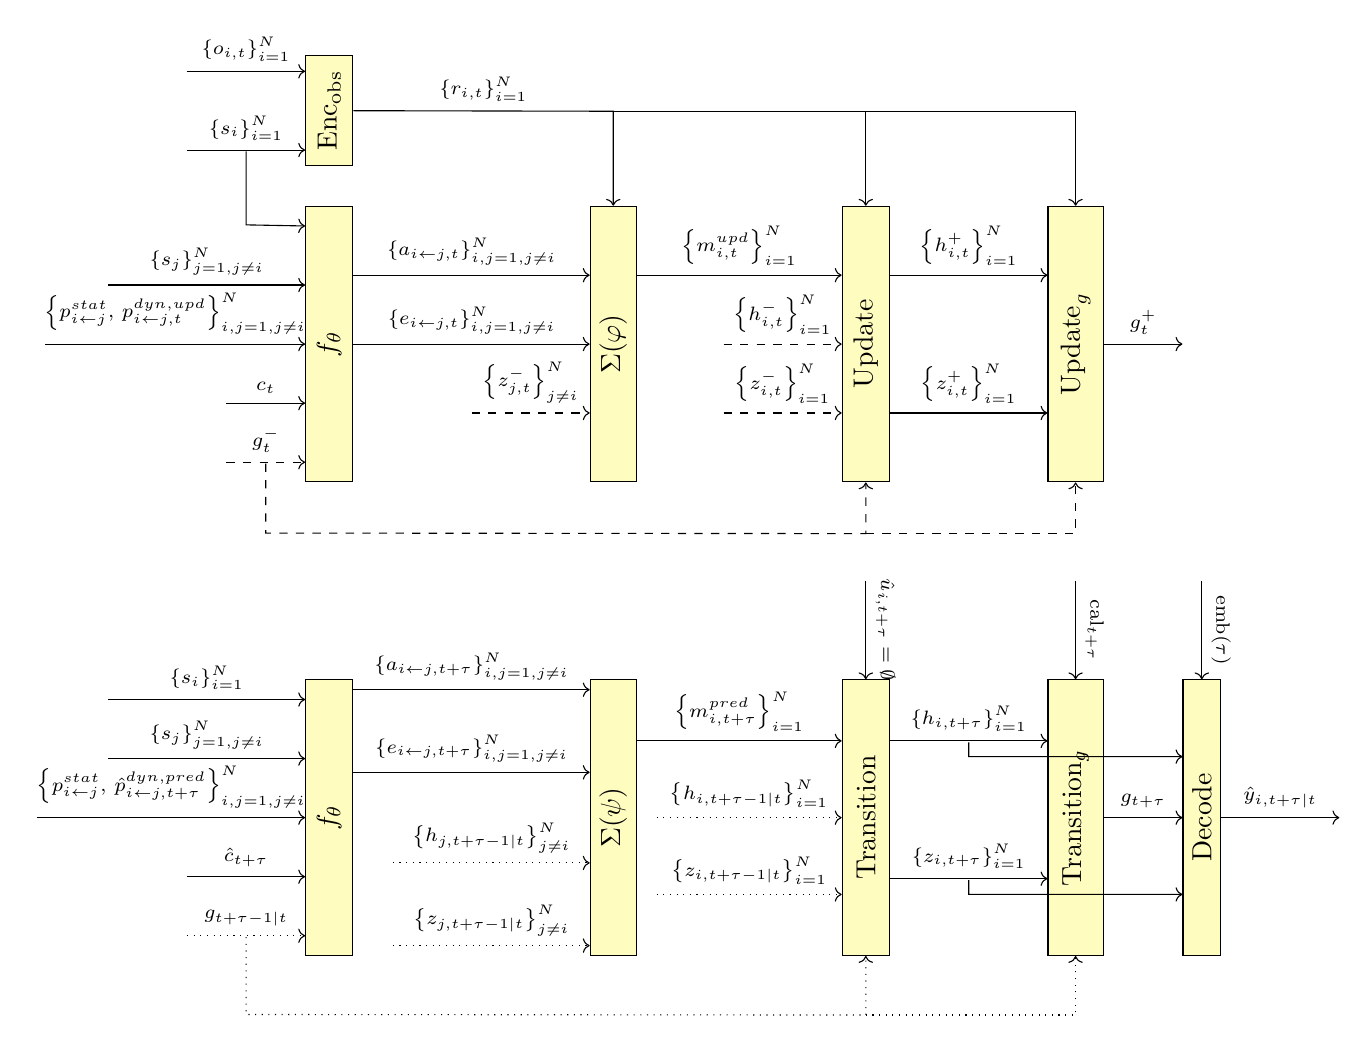
\begin{tikzpicture}[
    block/.style={ draw, fill=yellow!25 },
    edgelabel/.style={ midway, sloped, above, font=\scriptsize },
    branch/.style={ pos=0.5, inner sep=0mm, outer sep=0mm }
]

% Step A2
\node[block, minimum height=14mm, minimum width=6mm] (encobs) {\rotatebox{90}{$\mathrm{Enc}_{\mathrm{obs}}$}};
\draw[->] ($(encobs.west)+(-1.5,0.5)$) -- node[edgelabel] {$\left\{o_{i,t}\right\}_{i=1}^N$} ($(encobs.west)+(0,0.5)$);
\draw[->] ($(encobs.west)+(-1.5,-0.5)$) -- node[edgelabel] {$\left\{s_{i}\right\}_{i=1}^N$} node[branch] (branch) {} ($(encobs.west)+(0,-0.5)$);

% Step A3
\node[block, below=5mm of encobs, minimum height=35mm, minimum width=6mm] (ftheta) {\rotatebox{90}{$f_\theta$}};
\coordinate (p0) at ($(branch)+(0,-0.95)$);
\draw[->] (branch) --(p0)-- ($(ftheta.west)+(0,+1.5)$);
\draw[->] ($(ftheta.west)+(-2.5,0.75)$) -- node[edgelabel] {$\left\{s_{j}\right\}_{j=1,j\ne i}^N$} ($(ftheta.west)+(0,0.75)$);
\draw[->] ($(ftheta.west)+(-3.3,0)$) -- node[edgelabel] {$\left\{p^{stat}_{i\leftarrow j},\,p^{dyn,upd}_{i\leftarrow j,t}\right\}_{i,j=1,j\ne i}^N$} ($(ftheta.west)+(0,0)$);
\draw[->] ($(ftheta.west)+(-1,-0.75)$) -- node[edgelabel] {$c_{t}$} ($(ftheta.west)+(0,-0.75)$);
\draw[->, dashed] ($(ftheta.west)+(-1,-1.5)$) -- node[edgelabel] {$g_{t}^-$} node[branch] (branchgt) {} ($(ftheta.west)+(0,-1.5)$);

% Step A4
\node[block, right=30mm of ftheta, minimum height=35mm] (gmf) {\rotatebox{90}{$\Sigma(\varphi)$}};
\coordinate (p1) at ($(gmf.north)+(0,+12mm)$);
\draw[->] (encobs.east) -- node[edgelabel] {$\left\{r_{i,t}\right\}_{i=1}^N$} (p1) --  (gmf.north);
\draw[->] ($(ftheta.east)+(0,0.875)$) -- node[edgelabel] {$\left\{a_{i\leftarrow j,t}\right\}_{i,j=1,j\ne i}^N$} ($(gmf.west)+(0,0.875)$);
\draw[->] ($(ftheta.east)+(0,0)$) -- node[edgelabel] {$\left\{e_{i\leftarrow j,t}\right\}_{i,j=1,j\ne i}^N$} ($(gmf.west)+(0,0)$);
\draw[->, dashed] ($(gmf.west)+(-1.5,-0.875)$) -- node[edgelabel] {$\left\{z^-_{j,t}\right\}_{j\ne i}^N$} ($(gmf.west)+(0,-0.875)$);

% Step A5
\node[block, right=26mm of gmf, minimum height=35mm, minimum width=6mm] (update) {\rotatebox{90}{Update}};
\coordinate (p2) at ($(update.north)+(0,+12mm)$);
\draw[->] (p1) -- (p2) --  (update.north);
\draw[->] ($(gmf.east)+(0,0.875)$) -- node[edgelabel] {$\left\{m_{i,t}^{upd}\right\}_{i=1}^N$} ($(update.west)+(0,0.875)$);
\draw[->, dashed] ($(update.west)+(-1.5,0)$) -- node[edgelabel] {$\left\{h^-_{i,t}\right\}_{i=1}^N$} ($(update.west)+(0,0)$);
\draw[->, dashed] ($(update.west)+(-1.5,-0.875)$) -- node[edgelabel] {$\left\{z^-_{i,t}\right\}_{i=1}^N$} ($(update.west)+(0,-0.875)$);
\coordinate (p3) at ($(branchgt)+(0,-0.9)$);
\coordinate (p4) at ($(update.south)+(0,-0.65)$);
\draw[->, dashed] (branchgt) -- (p3) -- (p4) -- (update.south);

% Step A6
\node[block, right=20mm of update, minimum height=35mm, minimum width=7mm] (updateg) {\rotatebox{90}{$\mathrm{Update}_g$}};
\coordinate (p5) at ($(updateg.north)+(0,+12mm)$);
\draw[->] (p2) -- (p5) --  (updateg.north);
\draw[->] ($(update.east)+(0,0.875)$) -- node[edgelabel] {$\left\{h^+_{i,t}\right\}_{i=1}^N$} ($(updateg.west)+(0,0.875)$);
\draw[->] ($(update.east)+(0,-0.875)$) -- node[edgelabel] {$\left\{z^+_{i,t}\right\}_{i=1}^N$} ($(updateg.west)+(0,-0.875)$);
\coordinate (p7) at ($(updateg.south)+(0,-0.65)$);
\draw[->, dashed] (p4) -- (p7) -- (updateg.south);
\draw[->] (updateg) -- node[edgelabel] {$g_t^+$} ($(updateg.east)+(1,0)$);

% Step B1
\node[block, below=25mm of ftheta, minimum height=35mm, minimum width=6mm] (ftheta2) {\rotatebox{90}{$f_\theta$}};
\draw[->] ($(ftheta2.west)+(-2.5,1.5)$) -- node[edgelabel] {$\left\{s_{i}\right\}_{i=1}^N$} ($(ftheta2.west)+(0,1.5)$);
\draw[->] ($(ftheta2.west)+(-2.5,0.75)$) -- node[edgelabel] {$\left\{s_{j}\right\}_{j=1,j\ne i}^N$} ($(ftheta2.west)+(0,0.75)$);
\draw[->] ($(ftheta2.west)+(-3.4,0)$) -- node[edgelabel] {$\left\{p^{stat}_{i\leftarrow j},\,\hat p^{dyn,pred}_{i\leftarrow j,t+\tau}\right\}_{i,j=1,j\ne i}^N$} ($(ftheta2.west)+(0,0)$);
\draw[->] ($(ftheta2.west)+(-1.5,-0.75)$) -- node[edgelabel] {$\hat c_{t+\tau}$} ($(ftheta2.west)+(0,-0.75)$);
\draw[->, dotted] ($(ftheta2.west)+(-1.5,-1.5)$) -- node[edgelabel] {$g_{t+\tau-1|t}$} node[branch] (branchgtt) {} ($(ftheta2.west)+(0,-1.5)$);

% Step B2
\node[block, right=30mm of ftheta2, minimum height=35mm] (gmf2) {\rotatebox{90}{$\Sigma(\psi)$}};
\draw[->] ($(ftheta2.east)+(0,1.625)$) -- node[edgelabel] {$\left\{a_{i\leftarrow j,t+\tau}\right\}_{i,j=1,j\ne i}^N$} ($(gmf2.west)+(0,1.625)$);
\draw[->] ($(ftheta2.east)+(0,0.575)$) -- node[edgelabel] {$\left\{e_{i\leftarrow j,t+\tau}\right\}_{i,j=1,j\ne i}^N$} ($(gmf2.west)+(0,0.575)$);
\draw[->, dotted] ($(gmf2.west)+(-2.5,-0.575)$) -- node[edgelabel] {$\left\{h_{j,t+\tau-1|t}\right\}_{j\ne i}^N$} ($(gmf2.west)+(0,-0.575)$);
\draw[->, dotted] ($(gmf2.west)+(-2.5,-1.625)$) -- node[edgelabel] {$\left\{z_{j,t+\tau-1|t}\right\}_{j\ne i}^N$} ($(gmf2.west)+(0,-1.625)$);

% Step B3
\node[block, right=26mm of gmf2, minimum height=35mm, minimum width=6mm] (predict) {\rotatebox{90}{Transition}};
\draw[->] ($(gmf2.east)+(0,0.975)$) -- node[edgelabel] {$\left\{m_{i,t+\tau}^{pred}\right\}_{i=1}^N$} ($(predict.west)+(0,0.975)$);
\draw[->, dotted] ($(predict.west)+(-2.35,0)$) -- node[edgelabel] {$\left\{h_{i,t+\tau-1|t}\right\}_{i=1}^N$} ($(predict.west)+(0,0)$);
\draw[->, dotted] ($(predict.west)+(-2.35,-0.975)$) -- node[edgelabel] {$\left\{z_{i,t+\tau-1|t}\right\}_{i=1}^N$} ($(predict.west)+(0,-0.975)$);
\coordinate (p8) at ($(branchgtt)+(0,-1)$);
\coordinate (p9) at ($(predict.south)+(0,-0.75)$);
\draw[->, dotted] (branchgtt) -- (p8) -- (p9) -- (predict.south);
\draw[->] ($(predict.north)+(0,1.25)$) -- node[edgelabel] {$\hat{u}_{i,t+\tau}=\emptyset$} (predict.north);

% Step B4
\node[block, right=20mm of predict, minimum height=35mm, minimum width=7mm] (predictg) {\rotatebox{90}{$\mathrm{Transition}_g$}};
\draw[->] ($(predict.east)+(0,0.975)$) -- node[edgelabel] {$\left\{h_{i,t+\tau}\right\}_{i=1}^N$} node[branch] (branchhit) {} ($(predictg.west)+(0,0.975)$);
\draw[->] ($(predict.east)+(0,-0.775)$) -- node[edgelabel] {$\left\{z_{i,t+\tau}\right\}_{i=1}^N$} node[branch] (branchzit) {} ($(predictg.west)+(0,-0.775)$);
\coordinate (p11) at ($(predictg.south)+(0,-0.75)$);
\draw[->, dotted] (p9) -- (p11) -- (predictg.south);
\draw[->] ($(predictg.north)+(0,1.25)$) -- node[edgelabel] {$\mathrm{cal}_{t+\tau}$} (predictg.north);

% Step B5
\node[block, right=of predictg, minimum height=35mm] (decode) {\rotatebox{90}{Decode}};
\draw[->] (predictg) -- node[edgelabel] {$g_{t+\tau}$} (decode);
\coordinate (p12) at ($(branchhit)+(0,-0.2)$);
\draw[->] (branchhit) -- (p12) -- ($(decode.west)+(0,0.775)$);
\coordinate (p13) at ($(branchzit)+(0,-0.2)$);
\draw[->] (branchzit) -- (p13) -- ($(decode.west)+(0,-0.975)$);
\draw[->] ($(decode.north)+(0,1.25)$) -- node[edgelabel] {$\mathrm{emb}(\tau)$} (decode.north);
\draw[->] (decode) -- node[edgelabel] {$\hat{y}_{i,t+\tau|t}$} ($(decode.east)+(1.5,0)$);

\end{tikzpicture}
\end{figure}

\noindent 图中 $\hat c_{t+\tau}$ 统一表示未来窗使用的站点上下文简写，实际由模型内部解码得到的气象摘要 $\hat c^{met}_{t+\tau}$ 与已知未来日历 $\mathrm{cal}_{t+\tau}$ 拼接而成。

\newpage

\section{未来可能的方向}

\subsection{搜索增强}

我能不能先定义一组小而关键的未来不确定因素，再训练一个模块在这些候选情景里做排序？首先，测试 generator 是否真的有“oracle 可选性”，也就是说加入扰动生成大量轨迹之后，是否真的有至少一条轨迹可以比不加扰动的时候得到更低的 loss。价值网络的任务是，针对某个时间步的大量候选，找到未来具有最高潜力的那几个扰动结果（也就是 Q Search）。不过到底是先 Q Search 直接走还是先 Rollout 再 V Search 剪枝得实验过才知道。

\begin{itemize}
  \item 能不能先定义一组低维且关键的未来不确定因素（最好带一定物理语义），再由 generator 在这些候选情景上生成大量未来分支？
  \item 首先需要检验 generator 是否真的具有“oracle 可选性”：也就是说，对同一个样本生成大量候选轨迹之后，是否至少存在一条轨迹能比 baseline（即不加候选情景/不加修正时）取得更低的未来 loss。若不存在，则问题主要在 generator，而不在 scorer。
  \item 如果 oracle 可选性存在，那么再训练一个排序模块来从大量候选中选出未来最有潜力的那几个分支。
  \item 若采用 Q-search，则训练的是一个 Q 网络 / 候选评分器，用来对“当前状态 + 下一步候选方向”直接打分，从而在每个时间步的大量候选中先筛出 top-$K$ 分支。
  \item 若采用 V-search，则先将候选方向 rollout 一步得到子状态，再用 V 网络对子状态进行评估和剪枝。
  \item 至于最终采用“先 Q-search 预筛，再 rollout”，还是“先 rollout，再 V-search 剪枝”，需要通过实验比较其效果与计算代价。
  \item 一个关键实验指标是 oracle best-of-$K$ 相对 baseline 的提升幅度，它决定了后续 scorer / search 是否值得做。
\end{itemize}

\subsection{显式记忆为基础的时延传播}

\subsection{物理解释几个关键的矩阵}

\end{CJK}
\end{document}
